%\vspace*{\subsecspace}
%\section{SciSpot Design and Implementation}
%\section{Details of the Experimental Framework used for Evaluation}
\section{Implementing a Batch Computing Service For Preemptible VMs}
\label{sec:impl}

We have implemented a prototype batch computing service that implements various policies for constrained preemptions. 
We use this service to examine the effectiveness and practicality of our model and policies in real-world settings. 



Our service is implemented as a light-weight, extensible framework that makes it convenient and cheap to run batch jobs in the cloud. 
We have implemented our prototype in Python in about 2,000 lines of code, and currently support running VMs on the Google Cloud Platform~\cite{gcp}. 
%


Our service is implemented as a centralized controller, which implements the VM selection and job scheduling policies described in Section~\ref{sec:design}. 
The controller can run on any machine (including the user's local machine, or inside a cloud VM), and exposes an HTTP API to end-users. 
Users submit bags of jobs to the controller via the HTTP API, which then launches and maintains a cluster of cloud VMs, and maintains the job queue and metadata in a local database. 
%To improve usability, we automatically generate parameter combinations for a given bag size, based on a user-provided json file with ranges and constraints for each parameter. 

Our service integrates, and interfaces with two primary services.
First, it uses the Google cloud API~\cite{gcloud-api} for launching, terminating, and monitoring VMs.
Once a cluster is launched, it then configures a cluster manager such as Slurm~\cite{slurm} or Torque~\cite{torque}, to which it submits jobs. 
Our service uses the Slurm cluster manager, with each VM acting as a Slurm ``cloud'' node, which allows Slurm to gracefully handle VM preemptions.
The Slurm master node runs on a small, 2 CPU non-preemptible VM, which is shared by all applications and users. 
We monitor job completions and failures (due to VM preemptions) through the use of Slurm call-backs, which issue HTTP requests back to the central service controller. 

\noindent \textbf{Policy Implementation:}
Our service creates and manages clusters of transient cloud servers, manages all aspects of the VM lifecycle and costs, and implements the model-based policies.
It manages a cluster of VMs, and parametrizes the bathtub model based on the VM type, region,  time-of-day, and day-of-week.
When a new batch job is to be launched, it finds a ``free'' VM in the cluster that is idle, and uses the job scheduling policy to determine if the VM is suitable or a new VM must be launched.
Due to the bathtub nature of the failure rate, VMs that have survived the initial failures are ``stable'' and have a very low rate of failure, and thus are ``valuable''.
We keep these stable VMs as ``hot spares'' instead of terminating them, for a period of one hour. 
For the checkpointing policy, our dynamic programming algorithm has a time complexity of $O(T^3)$, for a job of length $T$.
To minimize this overhead, we precompute the checkpointing schedule of jobs of different lengths, and don't need to compute the checkpoint schedule for every new job.



\begin{figure}[t]
  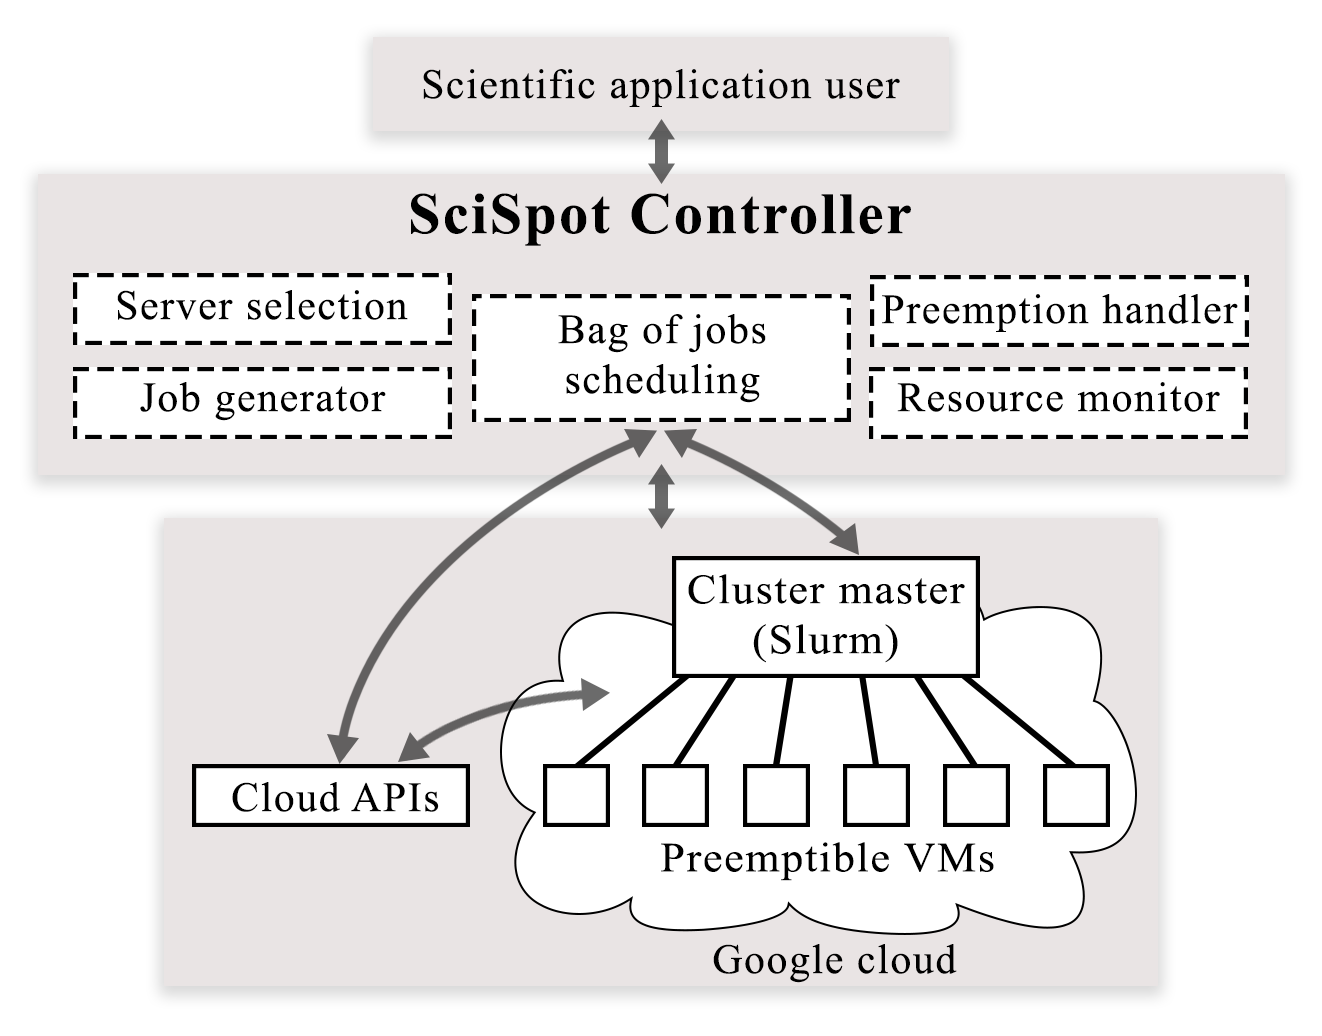
\includegraphics[width=0.3\textwidth]{../figures/Architecture.png}
\vspace*{\myfigspace}
  \caption{Architecture and system components of our batch computing service.}
  \label{fig:arch}
  \vspace*{\myfigspace}
\end{figure}


\noindent \textbf{Bag of Jobs Abstraction For Scientific Simulations:}
While our service is intended for general batch jobs, we incorporate a special optimization for scientific simulation workloads that improves the ease-of-use of our service, and also helps in our policy implementation. 
Our insight is that most scientific simulations involve launching a series of jobs that explore a large parameter space that results from different combinations of physical and computational parameters.

These workloads therefore can be abstracted as a ``bag of jobs'', with each job running the same application with slightly different parameters.
A bag of jobs is characterized by the job and all the different parameters with which it must be executed.
Within a bag, jobs show little varition in their running time and execution characteristics.


We allow users to submit entire bags of jobs, which permits us to determine the running time of the jobs, which we use in our scheduling and checkpointing policy.
Having a large sequence of jobs is also particularly useful with bathtub preemptions, since we can re-use ``stable'' VMs with low preemption probability for running new jobs from a bag.
If jobs were submitted one at a time, a batch computing service may have to terminate the VM after job completion, which would increase the job failure probability resulting from running on new VMs that have a high initial failure rate. 




% Additionally, our service also incorporates additional functionality to implement a ``bag'' of jobs that allows multiple jobs to be sequentially run.
% We observe that many batch jobs, especially scientific simulation workloads, do parameter sweeps. 

% Specifically, it runs a bag of jobs defined by these parameters:
% \begin{lstlisting}[basicstyle=\sffamily, frame=single, columns=fullflexible, escapeinside={(*}{*)}]
%   Bag of job = {(*$\mathcal{A}$*): Application to execute,
%   (*$n$*): Number of jobs,
%   (*$m$*): Minimum number of jobs to finish,
%   (*$\pi$*): Generator function for job parameters,
%   (*$\mathcal{R}$*): Computing resources per job}
% \end{lstlisting}


% We aim to provide a simple user interface to allow users to deploy their applications with minimum workflow changes. 

%Additionally, ease-of-use is one of \sysname's primary design goals, and we specifically incorporate

%it is suitable for running a large variety of applications.
% \sysname seeks to minimize the cost and running time of bags of jobs of scientific computing applications.
% \sysname's cost and time minimizing policies for running bags of jobs are based on empirical and analytical models of the cost and preemption dynamics of  transient cloud servers, which we present in the next section. 

% \noindent \textbf{High-level workflow:} When a user wishes to run a bag of jobs, \sysname handles the provisioning of a cluster of transient cloud servers.
% In addition, \sysname deals with the scheduling and monitoring of the bag of jobs, and with VM preemptions. 


% \sysname is designed as a framework that increases the usability and viability of transient cloud servers for scientific computing applications, and 
% Most scientific computing applications are deployed on HPC clusters that have a batch scheduler such as Slurm~\cite{slurm} or Torque~\cite{torque}, and \sysname integrates with these schedulers (e.g., Slurm) to provide the same interface to applications. 
% As shown in Figure~\ref{fig:arch},


%As part of \sysname, we also provide a base VM image with Slurm and MPI integration, along with commonly used libraries and benchmarks for scientific computing. To run an application, users must provide a location to the application source code or binaries. Integrating \sysname with container-based image management tools such as Docker~\cite{docker} and Singularity~\cite{kurtzer2017singularity} is part of our ongoing work. 





%%% Local Variables:
%%% mode: latex
%%% TeX-master: "paper"
%%% End:
